\chapter{Developing the Conceptual Framework}
\label{chap-framework}

The preliminary evaluations investigate what makes effective developer recommendations by exploring the effectiveness of peer interactions and the failures of the \tele. Altogether, these studies posit four \textit{developer recommendation preconditions}, or aspects necessary to make effective recommendations to programmers, \textbf{desire}, \textbf{familiarity}, \textbf{social context}, and \textbf{developer workflow}. However, as opportunities for peer interactions decline and bots produce inadequate suggestions, how can these prerequisites be incorporated into automated recommendations to encourage developer behaviors? This chapter introduces \FRAMEWORK, a state-of-the-art approach to design automated systems by presenting desirable and informative recommendations to developers within their development environment and workflow.


\section{Developer Recommendation Choice Architectures}

Choice architecture refers to the organization of the context in which humans make decisions~\cite{thaler2013choice}. To improve the decision-making of humans, Johnson and colleagues posit 11 practical tools for choice architects, or ``anyone who present(s) people with choices'', valuable for structuring decisions and describing options to encourage the adoption of target behaviors~\cite{johnson2012beyond}. In this work, I view software engineering researchers and toolsmiths are also \textit{choice architects}, creating tools and practices requiring developers to make decisions while developing and maintaining software applications. Thus, I argue the presentation and organization of these decisions to developers impacts the choices they make in their work.

% the developer behavior adoption problem  

To further improve software engineering bots, I introduce \FRAMEWORK, a conceptual framework to design automated recommendations from bots. This approach is motivated by the findings from the preliminary studies (Chapter~\ref{chap-peer}), software engineering literature, and prior work in nudge theory. To devise this framework, I analyzed the tools for choice architecture and apply these concepts in a development context. This mapping, presented in Table~\ref{tab:framework}, derived three principles for designing developer recommendations: \textbf{\em actionability}, \textbf{\em feedback}, and \textbf{\em locality}. By incorporating these concepts into automated notifications, we can improve the way decisions are presented to developers and encourage adoption of useful tools and practices. For the remainder of this chapter, we provide definitions, motivation, and example for each principle and present a formative evaluation of this framework exploring actionable recommendations.

\newgeometry{margin=1in}
\begin{landscape}
\thispagestyle{empty}
\begin{table*}
%/centering
\caption{Developer Recommendation Choice Architectures}
    \begin{tabular}{ |l|l|l| }
	\hline
	\textbf{} & \textbf{Choice Architecture Tool~\cite{johnson2012beyond}} & \textbf{Definition} \\
	\hline
	\multirow{2}{*}{\textbf{\em Actionability}} 
	 & Technology and decision aids & Introducing technology to aid decision makers in choice tasks \\ \cline{2-3}
	 & Use defaults & The way decision makers initially encounter choice tasks \\ \hline
	\multirow{6}{*}{\textbf{\em Feedback}}
	 & Reduce number of alternatives & Limiting the number of choice options presented to decision makers \\ \cline{2-3}
	 & Focus on satisficing & Helping users consider outcomes that lead to higher choice satisfaction \\ \cline{2-3}
	 & Attribute parsimony and labeling & Limiting the number of characteristics presented with options \\ \cline{2-3}
	 & Translate and rescale for better evaluability & Presenting attributes to increase impact and clarity \\ \cline{2-3}
	 & Customized information & Personalization to account for individual differences between decision-makers \\ \cline{2-3}
	 & Focus on experience & Considering the background and knowledge of decision-makers \\ \hline
	\multirow{3}{*}{\textbf{\em Locality}}
	 & Limited time windows & Providing time restrictions for users to make decisions \\ \cline{2-3}
	 & Partitioning of options & Groups or categories of options or attributes \\ \cline{2-3}
	 & Decision staging & Dividing decisions into multiple stages \\ \hline 
\end{tabular}
\label{tab:framework}
\end{table*}
%\vfill
\raisebox{-8.646cm}{\makebox[\linewidth]{\thepage}}
\end{landscape}
\restoregeometry

\subsection{Actionability} 

Actionability refers to the ease with which developers can adopt behaviors presented in recommendations. Nudge theory research suggests actionability is a key concept for encouraging humans to make better decisions. For example, Thaler and Sunstein suggest a simple nudge is to make target behaviors easy to apply because ``many people will take whatever option requires the least effort, or the path of least resistance''~\citep[p.~85]{nudge}. Similarly, Johnson suggests incorporating technology aids and using defaults are actionable ways to influence human behavior. For example, Madrian and Shea implemented the default rule to nudge employees to enroll in retirement plans. By having users automatically opt-in to 401k plans instead of requiring manual signing up, they discovered increased enrollment, with 98\% of new employees selecting a plan within 36 months, and improved money-saving behaviors~\cite{madrian2001power}. 

In the \tele evaluation, we found developers disapproved of recommendations from \toolone because of their deficiencies integrating into development workflows and making more work for developers. For example, P3 commented ``This introduces a bunch of errors, can you check whether they are worth fixing or configure the plugin so as to ignore the false positives?''. Software engineering research also shows actionability is important to developers for adopting development tools and practices. For instance, Heckman and colleagues examined the concept of actionability through static analysis notifications in AAITs (actionable alert identification techniques) to help developers identify and resolve defects~\cite{Heckman11Actionable}. Additionally, Evans and colleagues show that by automatically turning on security analyses in the \textsc{Split} static analysis tool\footnote{\url{https://splint.org/}} increased the amount of security vulnerabilities fixed~\cite{evans2002splint}. We propose actionable development tool and behavior recommendations can increase adoption from developers.

\subsection{Feedback} 

The feedback principle refers to providing clear and relevant information to developers. Sunstein and Thaler note ``the best way to help Humans improve their performance is to provide feedback'' and ``choices can be improved with better and simpler information''~\citep[p.~92,~204]{nudge}. Johnson suggests practical techniques for improving feedback to decision-makers during choices such as limiting the number of options, presenting desirable outcomes, adding labels, reducing the attributes of choices, providing comprehensible content for choosers to evaluate, customizing information and messages, and relating to knowledge and experiences~\cite{johnson2012beyond}. Behavioral science research shows enhanced feedback on decisions improves human behavior. For instance, most people order familiar and repeated meals at fast food restaurants, however nudges such as providing information on the amount of calories in food and customized recommendations for daily caloric intake encouraged consumers to purchase unfamiliar and healthier meals~\cite{Wisdom2010Healthy}.

The results from the peer interactions study suggest providing information about desirable outcomes and targeting familiar concepts of tools and behaviors can incorporate receptiveness into recommendations. Similarly, the \tele study found generic and irrelevant recommendations from \toolone were unproductive, violating social context, and respondents longed for details that ``\textit{would actually help}'' and ``\textit{attach[ing] a report with actual findings in our code instead of just some generic example}'' (P7). Software engineering research also suggests feedback to developers factors in influencing their behavior. For instance, Barik and colleagues examined the structure of compiler error messages on how developers resolved problems~\cite{barik2018should}. Furthermore, Cerezo and colleagues suggest that \textit{user-driven communication} can improve the perception of chatbots compared to bot-driven techniques~\cite{cerezo2019building}. To improve the effectiveness of automated recommendations to software engineers, we believe providing useful information and feedback will improve the likelihood developers adopt useful behaviors.

\subsection{Locality} Locality refers to the setting of recommendations in the context of developers completing programming tasks. Johnson presents several tools for incorporating choice architecture into the setting of choices, including restricting the amount of time for users to make decisions, organizing options into groups, and dividing decisions into multiple states~\cite{johnson2012beyond}. Prior work studying RSSEs also suggests \textit{when} and \textit{what} to recommend are challenges for automated recommender systems~\cite{happel2008challenges}. To describe locality in recommendations for developers, we divide this concept into two subcategories: \textit{spatial} and \textit{temporal} locality.

\subsubsection{Spatial:} Spatial locality refers to the location where developer receive recommendations. Behavioral science research suggests the location of options matters when encouraging humans to adopt beneficial behaviors. For example, Hanks found that by changing the location of vegetables and fruits in a high school cafeteria, they found an increase in the amount of healthier foods purchased and consumed by students~\cite{Hanks2012Lunchroom}. The preliminary studies also suggest location matters in recommendations. For example, in the peer interactions study a participant recommended the Find and Replace functionality in Excel and their partner responds ``\textit{Where's the find and replace?}'' (S12), displaying their unfamiliarity with the feature. 

Software engineering research shows the placement of decisions impacts the behavior of programmers, as developers prefer notifications located in convenient locations. For example, in a collaboration with Smith et al. we developed \textsc{Flower}, an Eclipse code navigation plugin created to help developers avoid disorientation by incorporating \textit{in situ} design principles to prevent users switching between views during code search. We found the location of suggestions within the coding editor of the IDE led to increased efficiency with branchless navigation for developers to find security vulnerabilities and received positive feedback from participants~\cite{Flower}. Thus, I propose automated recommendation systems for encouraging developer behaviors should situate suggestions in convenient and detectable locations to improve the decision-making of software engineers.

\subsubsection{Temporal:} Temporal locality refers to the timing of recommendations made to developers. Nudge theory suggests timing of decisions influences human decision-making. For example, an effective nudge for farmers in Kenya was to change the time of year for fertilizer discounts, and this time-limited window encouraged them to make purchases earlier and improve the harvest of crops~\cite{duflo2011nudging}. In the \tele study, developers mentioned the potential impact of adopting \toolone recommendations on the timing of their project builds led to ineffective recommendations. For example, P7 desired information about ``\textit{the over head in terms of build time}''. These naive recommendations also came at inconvenient times for developers who did not have the bandwidth to fix additional issues and breaking builds, such as one respondent who commented, ``\textit{Can you fix the errors reported by your tool in the build so that I can see the proposed changes?}'' (P17).

Software engineering research also shows that the timing of recommendation within programmers' workflow is important for increasing adoption of developer behaviors. For example, Distefano examined configuring static analysis tools to run at \textit{diff time}, or on code contributions submitted by developers during code review before being merged into the code base, and found that this rescheduling increased the fix rate of reported bugs up to 70\% compared to nearly 0\% for times outside the development workflow, such as assigning bug lists to developers overnight~\cite{Distefano2019Facebook}. Alternatively, untimely recommendations led to programmers ignoring code navigation strategies from Spyglass~\cite{viriyakattiyaporn2009challenges}. To improve the effectiveness of automated recommendations, systems should make timely suggestions to programmers within their workflow to increase their desire to adopt useful software engineering behaviors and practices.



\section{Preliminary Evaluation}

To explore the impact of \framework on the behavior and decision-making of software engineers, I conducted a preliminary evaluation to provide an overview of actionable recommendations. While this work focuses solely on \textit{actionability}, the subsequent studies and future work aim to study all of the conceptual framework principles.

\subsection{Methodology}

To evaluate actionability in automated recommendations, this study incorporates multiple methods of analyzing survey responses to quantitatively evaluate developer preferences and qualitatively collect feedback on actionable recommendations.

\subsubsection{Data Collection}

\paragraph*{Participants}

Professional software engineers were recruited to participate in this study. Overall, we received responses from 15 software developers and participants had an average of 7.3 years of industry programming experience. 

\paragraph*{Study Recommendation}

For this evaluation, we presented participants with recommendations to fix a \texttt{PEP 3105} Python 3 style warnings. This warning indicates Python \texttt{print} statements are are now \texttt{print()} functions in the latest version of the programming language.\footnote{\url{https://www.python.org/dev/peps/pep-3105/}} For instance, line 9 of Listing~\ref{listing:pep} contains an example \PEP violation. This simple recommendation also has larger implications for improving the behavior of developers because, as of January 1, 2020, Python 2 is officially no longer supported. The programming language announced there will be ``no new bug reports, fixes, or changes'' to the older version and encouraged developers to upgrade to Python 3.\footnote{\url{https://www.python.org/doc/sunset-python-2/}} Our sample recommendations proposed fixing \PEP warnings and upgrading the code base to Python 3.

\paragraph*{Survey}

To investigate the impact of actionability in automated suggestions, we presented participants with sample automated recommendations to fix \PEP warnings and upgrade to the latest version of Python. The survey presented participants with screenshots of two suggestions, one actionable and one static, and asked participants to select which recommendation they preferred and provide reasoning behind their choice. Additionally, we asked participants to input their years of professional development experience and to provide general feedback on designing automated recommendations from bots. The survey distributed to developers is available to view in Appendix~\ref{app-sorry2-survey}.

\begin{listing}
\centering
 \caption{Example of a \PEP static analysis violation and fix}{}
\begin{minted}[xleftmargin=6cm,fontsize=\small,linenos,firstnumber=9]{python}
if status is True:
-   print 'passed'
+   print('passed')
\end{minted}
\label{listing:pep}
\end{listing}


\subsubsection{Determining the effectiveness of actionable recommendations}

In this formative evaluation, we surveyed developers to investigate actionability in automated recommendations. The survey included actionable and static recommendations to fix \PEP errors and a message encouraging users to upgrade from Python 2 to Python 3. The static recommendation presented to participants is displayed in Figure~\ref{fig:sorry2-static}, while Figure~\ref{fig:sorry2-action} presents the actionable recommendation. Based on the \framework design principles, both of these recommendations incorporate the same \textit{feedback} (information to promote repairing the \PEP error, proposing a fix, and encouraging users to upgrade to Python 3), \textit{spatial locality} (placed on Line 10 of a sample code snippet containing a \PEP error), and \textit{temporal locality} (located on an open pull request before the code is merged). 

\begin{figure}[H]
\centering
	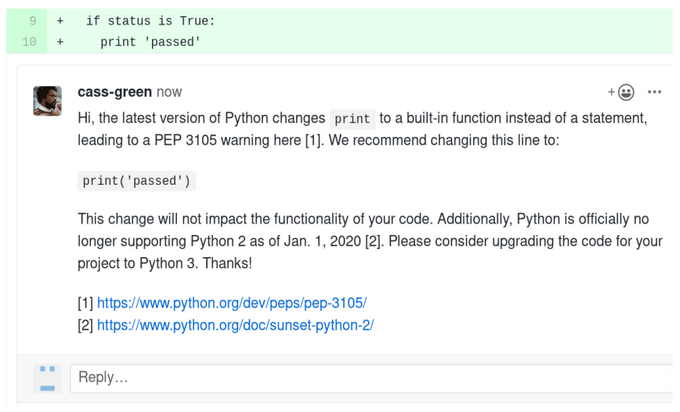
\includegraphics[width=0.8\textwidth]{Chapter-4/images/static.png}
	\caption{Static recommendation to fix a \PEP error}
	\label{fig:sorry2-static} 
\end{figure}

\begin{figure}[H]
\centering
	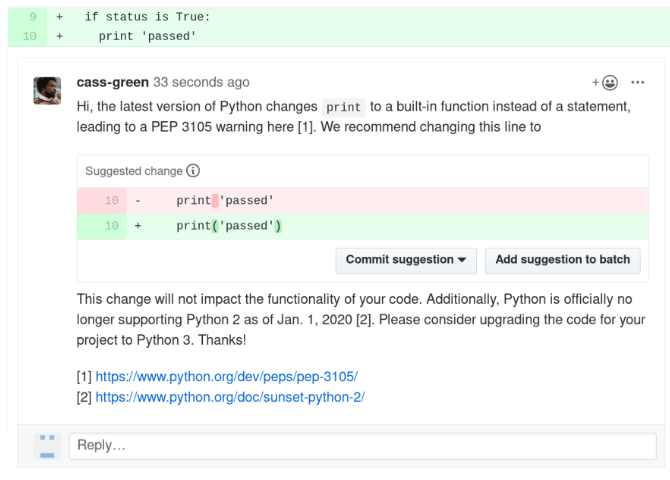
\includegraphics[width=0.8\textwidth]{Chapter-4/images/actionable.png}
	\caption{Actionable recommendation to fix a \PEP error}
	\label{fig:sorry2-action} 
\end{figure}

\newpage
However, these sample notifications differ on the \textit{actionability} of recommendations. The static recommendation would require developers to re-submit a pull request to make the proposed change (\texttt{print('passed')}). On the other hand, the actionable recommendation incorporates a ``Commit suggestion'' button which allows developers to automatically commit the suggested fix for the \PEP violation to their code. This technology aid makes the decision of whether or not to fix the error simpler for developers by providing a solution and incorporating the ability to easily integrate the suggested code changes into their workflow and code. We aim to discover how this design decision impacts developers' preferences for adopting behaviors from automated recommendations.

\subsection{Results}

Our survey responses, presented in Table~\ref{tab:results}, reveal 100\% of developers ($n = 15$) preferred the actionable recommendation over the static approach. This indicates developers are much more likely to adopt recommendations that make it easier to adopt suggestions. Developers also provided feedback praising the actionable recommendation, reporting it ``\textit{lets you automatically merge it}'' (P8), ``\textit{appl[ies] the change automatically}'' (P3), ``\textit{provide[s] an actionable short cut}'' (P2), and ``\textit{can directly commit the change instead of having to do a manual commit}'' (P10). Thus, we conclude that actionability is an effective approach for encouraging developers to improve their behavior. 

\begin{table}[htbp]
    \centering
    \caption{Survey Results on the Actionability of Recommendations}
    \begin{tabular}{|c|c|c|} \hline
          & \textbf{\em n} & \textbf{Percent}\\ \hline
         static & 0 & 0\% \\ \hline
         actionable & 15 & 100\% \\ \hline
    \end{tabular}
    \label{tab:results}
\end{table}

\section{Discussion}

To improve developer decision-making, I present \framework, a conceptual framework which incorporates concepts from nudge theory to design actionable, informative, and convenient automated recommendations. This approach, motivated by the preliminary studies exploring effective developer recommendations as well as prior work in behavioral science and software engineering, posits \textit{actionability}, \textit{feedback}, and spatial and temporal \textit{locality} as key factors influencing the adoption of developer behaviors. As choice architects, software engineering researchers and bot developers can enhance the way decisions are presented to programmers by integrating this framework into automated recommendation systems. To evaluate this approach, I conducted a formative evaluation investigating the impact of actionability on developers' perception of automated recommendations, and found participants significantly prefer actionable notifications in contrast to static ones. By incorporating this framework into automated recommendations, the thesis of this dissertation argues that systems can encourage the adoption of behaviors useful for improving code quality and productivity of developers (Chapter~\ref{chap-thesis}). The next two chapters present further evaluations of \framework by analyzing existing recommender systems (Chapter~\ref{chap-suggs}) and introducing new tools incorporating this framework (Chapter~\ref{chap-bot}) to analyze its impact on the decision-making and behavior of developers.

